We will in this chapter characterize the fluctuations.

As seen in \cref{fig:2DFluct}, the fluctuations can be quite strong.
This is something which has also been observed experimentally in for example \cite{Burin2005}.
To get a better feeling of how strong the fluctuations are, we can compare the steady state profiles with the turbulent profiles.
\Cref{fig:posOfFluct01} gives such a comparison.
%
\begin{figure}[h!]
    \begin{center}
        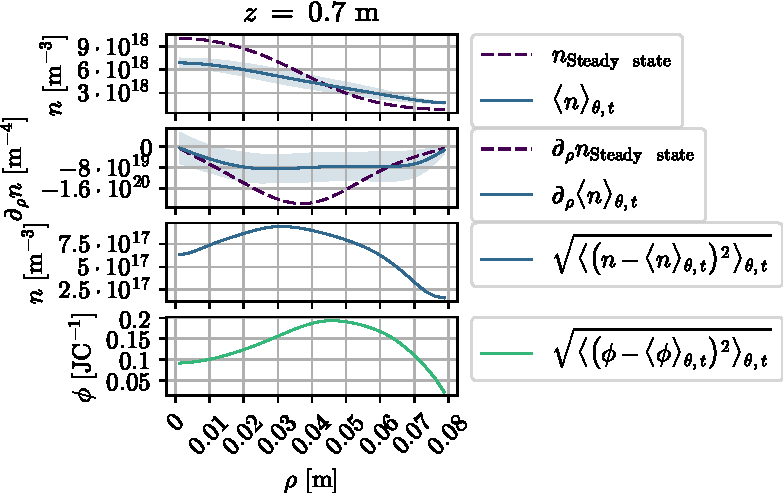
\includegraphics{fig/results/posOfFluct/posOfFluctB01}
    \end{center}
    \caption{Flattening of the profiles together with the position of the fluctuations for $B=0.1\T$.
        The subscripted $_\text{Steady state}$ denotes steady state variables, whereas variables without subscript denotes quantities in the saturated turbulence phase.
        A poloidal and temporal average (containing the whole time series) have been done in order to get a good avergaged picture of the turbulent profile.
        The shaded area represents the standard deviation.
    }
    \label{fig:posOfFluct01}
\end{figure}
%
Other than noting that the amplitude of the fluctuations are the largest around the maximum gradient, we observe the background profiles gets flattened by the turbulence.
This is an important feature which need to be considered when modelling the plasma.

In models like Hasegawa-Wakatani \cite{Hasegawa1987,Holland2007}, the fluctuations are separated from the mean (a so-called Reynolds decomposition).
The model only evolves the fluctuation in time, whilst keeping the mean fixed as a static background.
In such models, the free energy in the background gradients are driving the fluctuations, and the feedback of the fluctuation on the background profiles are neglected.
Such a approximation is good if the fluctuations are small.
On the other hand, if the fluctuations are large as in \cref{fig:posOfFluct01}, the background gradients are altered, and thus the drive for the fluctuations.

A global approach which doesn't uses the Reynolds decomposition is therefore needed.
With such a global approach, the change in the driving force for the turbulence is accounted for, and it enables one to investigate the backreaction to the background from the fluctuations.
Models like CYTO \cite{Naulin2008,Windisch2011a,Windisch2011b} and CELMA are using such a global approach.

Further investigation of the turbulence can be done by investigating the fluctuations at a fixed point.
This is done in \cref{fig:combinedPlots008}, where the tim trace, the probability density function (PDF) and power spectra density (PSD) is shown at $3$ different radial positions.
%
\begin{figure}[htb]
    \centering
    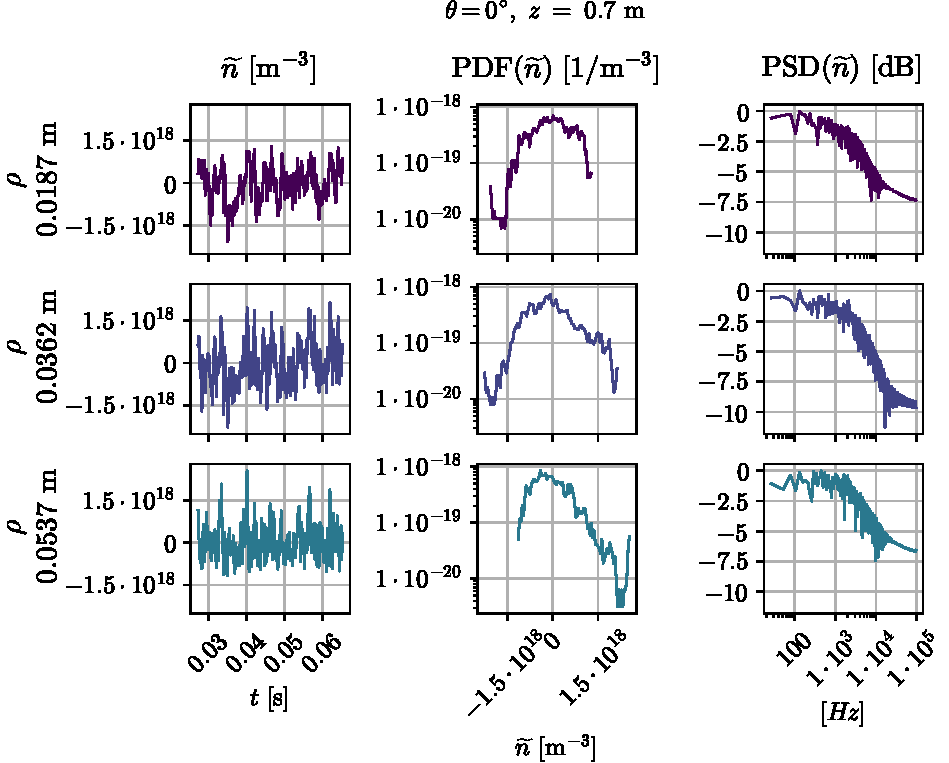
\includegraphics[width=1.0\textwidth]{fig/results/combinedPlots/008T}
    \caption{Characteristics of the time traces of the fluctuations at three radial positions.
        The top row shows data probed close to the axis of the cylinder,
        the middle row shows data probed at position of the highest density gradient,
        and the bottom shows data probed close to the edge of the plasma.
    }
    \label{fig:combinedPlots008}
\end{figure}
%
Again, we can observe that the fluctuations are large in amplitude, and increasingly intermittent for higher radius.
The power spectra density (PSD) shows that several frequencies are present simultaneously, and that the system is more turbulent at the edge.
This behavior is captured by the probability density functions (PDF), which measures the chance to encounter a value within an infinitesimal range, if a value at a random time is withdrawn from the time trace.
Consequentially, if all values are equally probable, the PDF will have a Gaussian shape.
Deviations from the Gaussian shape is usually measured by the statistical moments skewness $S$%
%
\footnote{
    The skewness is a measure of the mass of the distribution.
    If the skewness is negative, the left tail of the distribution is bigger than the right.
    For a pure Gaussian the skewness is 0.
}
%
and kurtosis $K$
%
\footnote{
    The kurtosis is a measure of extreme events present in the distribution.
    For a pure Gaussian the skewness is 3.
    If the kurtosis is less than 3 (platykurtic) the distribution produces fewer and less extreme outliers than a Gaussian.
    If the kurtosis is greater than 3 (leptokurtic) there are more extreme outliners, and the tails approaches zero slower than a Gaussian.
}
%
defined as
%
\begin{align*}
    &S=E\L[\L(\frac{X - \mu_X}{\sigma_X}\R)^3\R]&
    &K=E\L[\L(\frac{X - \mu_X}{\sigma_X}\R)^4\R],
\end{align*}
%
where $E$ denotes the expectiation value operator, $\mu_X$ the mean of $X$, and $\sigma_X$ the standard devitaion%
\footnote{We are assuming that the tail of the distribution are approaching fast enough to $0$ in order for the moments to be defined.}
.
Figure \cref{fig:skewKurt008} highlights how this varies with the radius.
%
\begin{figure}[htb]
    \centering
    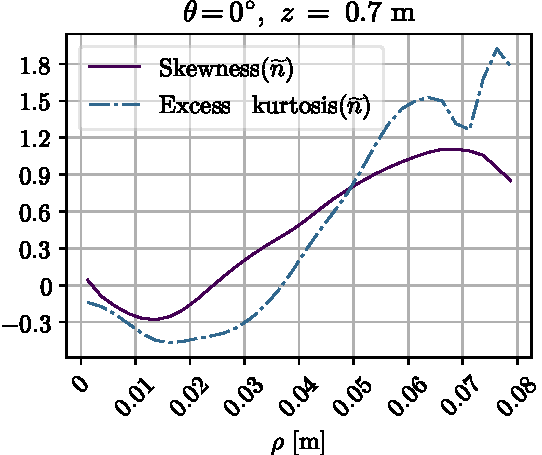
\includegraphics{fig/results/skewKurt/008T}
    \caption{Radial variations of the skewness and excess kurtosis (the kurtosis $-3$).}
    \label{fig:skewKurt008}
\end{figure}
%

One can see that close to the center, it is more probable to encounter a negative fluctuation than a positive fluctuation.
Then, for higher radii, large positive fluctuations becomes more and more frequent.
From the excess kurtosis, we can see that extreme events are less likely than in a Gaussian random process, whereas extreme events are almost twice as likely in the edge as in a Gaussian random process.

We will proceed by investigating two of our observations further.
First, from our phenomenological discussion in \cref{sec:simpleLin} (which is shown mathematically in for example in \cite{Garcia2001a}), a large positive fluctuations in the density is not enough to give a positive flux.
The flux is obly obtained when there is a phase shift between the density and the potential.
Therefore, we would like to investigate the turbulent flux particle in the next section.
After that, we will investigate the intermittency of the signal, and search for blobs and holes.
